\documentclass[12pt]{article}
%\usepackage[UTF8]{ctex}
\usepackage[tc]{titlepic}
\usepackage{titlesec}
\usepackage{cite}
\usepackage{fancyhdr}
\usepackage{booktabs}
\usepackage{float} 
\usepackage{graphicx} 
\usepackage{amsmath}
\usepackage{multirow}
\usepackage{amssymb}
\usepackage{amsthm}
\usepackage{mathrsfs}
\usepackage{bm}
\usepackage{tikz}
\usepackage{comment}
\usepackage{pgfplots}
\pgfplotsset{compat=1.18}
\usetikzlibrary{arrows.meta, positioning, shapes.geometric}
\usepackage{mhchem}
\usepackage{siunitx}
\usepackage[section]{placeins}
\usepackage{caption}
\usepackage{xcolor}
\usepackage{listings}
\usepackage{hyperref}
\usepackage{graphicx}
\usepackage{geometry}
\usepackage[section]{placeins}
\geometry{a4paper,scale=0.8}
\pagestyle{fancy}
\title{1}

\lstset{
language=R,
basicstyle=\color{gray}\ttfamily\small 
}

\begin{document}

\section{description}
\textbf{still trying to express $f_s$ and $f_e$ in a better way}\\
Let $p$ denote fraction of infected patches and $N$ denote population density of infected patches. 
\begin{figure}[H]
\centering
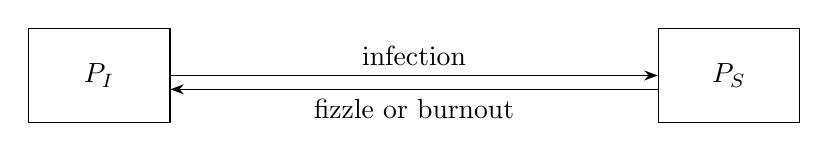
\begin{tikzpicture}[
  node distance=4cm and 3cm,
  every node/.style={align=center},
  box/.style={draw, minimum width=1.8cm, minimum height=1.2cm},
  >={Stealth}
]
% Nodes   
\node[box] (I) at (0:4) {$P_S$};  
\node[box] (S) at (180:4) {$P_I$};  
% Arrows
\draw[->] (S) -- node[above] {infection} (I);
\draw[->, transform canvas={yshift=-5pt}] (I) -- node[below] {fizzle or burnout} (S);
\end{tikzpicture}
\caption{patch state transition}
\end{figure}
\textbf{spread:}
Hosts move around and simultaneously bring pathogens to susceptible patches (combining movement and infection in one step to avoid calculating average density again)
$$f_s:\begin{pmatrix}
    p\\N
\end{pmatrix}
\to \begin{pmatrix}
    p+Bp(1-p)\\
    N+c(1-p)(S-N)
\end{pmatrix}$$
$B$ is infection rate (currently setting $B$ as constant
since we've already set $R_0$ as constant too), $c$ is moving probability of individual rats, and $S$ is the population density of susceptible patches (assumed constant).\\

\textbf{epidemic:}
Infected hosts die and so some infected patches burnout. 

$$f_e:\begin{pmatrix}
    p\\N
\end{pmatrix}
\to \begin{pmatrix}
    P_1p\\
    (1-zD)N
\end{pmatrix}$$
$P_1$=
\lstinline{P1_prob(N)} is the persistence probability, $z$ is final size of this epidemic wave, $D$ is the death probability of infected hosts. \\

\textbf{growth:}
Assume a constant birth rate $r$.
$$f_g:\begin{pmatrix}
    p\\N
\end{pmatrix}
\to \begin{pmatrix}
    p\\
    (1+r)N
\end{pmatrix}$$
\\

The overall iteration process is
$$f=f_g\circ f_e\circ f_s:\begin{pmatrix}
    p\\N
\end{pmatrix}
\to \begin{pmatrix}
    P_1(p+Bp(1-p))\\
    (1+r)(1-zD)(N+c(1-p)(S-N))
\end{pmatrix}$$
where 
$P_1$=
\lstinline {P1_prob(N+c(1-p)(S-N))}
    
\section{range of parameters}
Consider quadratic function $y=x+kx(1-x)$ where $0\leq x\leq 1$ and $k\geq 0$,
$$f(x)=x+kx(1-x)=-kx^2+(k+1)x, x \in R $$

We want to make sure that $f([0,1])\subset [0,1]$. The function attains its maximum at $x^*=\frac{k+1}{2k}$. Note that $f(0)=0$ and $f(1)=1$, so we'll need to require that $x^*\geq1$, i.e. $0\leq k\leq1$. \\
\begin{itemize}
    \item \textbf{infection}:  $p\leftarrow p+Bp(1-p)$, we require $0\leq B\leq1$
    \item \textbf{burnout}: $p=P_1p$, $0\leq P_1 \leq 1$
    \item \textbf{epidemic}: $0\leq z \leq1$ and $0\leq D \leq 1$
    \item \textbf{movement:} $0\leq c \leq 1$
    \item \textbf{birth}:  $(1+r)(1-zD)\leq 1$
\end{itemize}

\section{Disease Free Equilibrium}
If we start at a point where $p>0,N>0$, all variables remain positive during the iterations as each step maps positive values to a positive values. \\
If we start at $p=0,N>0$  then population size ends up at  
$$
N_t=N_{t+1}=(1+r)(1-zD)(N_t+(p-1)(S-N_t))
$$
i.e.
$$N_{DFE}=\frac{c(1+r)(1-zD)S}{1-(1+r)(1-zD)(1-c)}$$
$N_{DFE}$ increases with $r,c,S$ and decreases with $z,D$.
\section{invasion analysis}
$$
    J_{f_s}=\begin{pmatrix}
    1+B-2Bp&0\\-c(S-N)&1
\end{pmatrix}
$$\\
$$
    J_{f_e}=\begin{pmatrix}
P_1&p\frac{\partial P_1}{\partial N}\\0&1-zD
\end{pmatrix}$$
\\
$$
    J_{f_g}=\begin{pmatrix}
1&0\\0&1+r
\end{pmatrix}
$$
And at DFE we have $p=0,N=N_{DFE}$ so the matrices above are all lower triangular, so eigenvalues of $J_f=J_{f_g}J_{f_s}J_{f_e}$ 
are $e_1=(1+B)P_1$ and $e_2=(1-zD)(1+r)$. We required previously that $e_2$ is always smaller than 1. If $(1+B)P_1|_{N=N_{DFE}+c(S-N_{DFE})}<1$, DFE is stable, so the disease cannot persist; if it is greater than 1, DFE is unstable, the disease will persist and system ends up at endemic equilibrium.

\section{Endemic equilibrium}
Endemic equilibrium indicates
\begin{align*}
    &P_1(1+B(1-p))=1\\
    &(1+r)(1-zD)(N+c(1-p)(S-N))=N
\end{align*}
$$P_1=p_k(1-q(x_{in})^{y \star(N+c(1-p)(S-N)})$$
$p_k,q(x_{in}),y \star$ are all defined in burnout paper. Denote $\frac{1}{(1+r)(1-zD)}=t$ then we get $N+c(1-p)(S-N)=tN$ and $1-p=\frac{N(t-1)}{c(S-N)}$. Plug this into first equation and we get
$$(1-\mathrm{e}^{ty_\star \ln q(x_{in})N)}(1+\frac{BN(t-1)}{c(S-N)})=\frac{1}{p_k}$$
i.e.,
$$\mathrm{e}^{ty_\star \ln q(x_{in})N}\frac{N-\frac{cS}{c-B(t-1)}}{N-\frac{cS(p_k+1)}{c(p_k+1)-p_kB(t-1)}}=\frac{p_kB(t-1)-c(p_k+1)}{p_k(B(t-1)-c)}$$
denote $w=ty_\star \ln q(x_{in}),u=\frac{cS}{c-B(t-1)},v=\frac{cS(p_k+1)}{c(p_k+1)-p_kB(t-1)},a=\frac{p_kB(t-1)-c(p_k+1)}{p_k(B(t-1)-c)}$ 
Then the equation is
$$\mathrm{e}^{wN}\frac{N-u}{N-v}=a$$
The solution is 
\begin{align*}
&N^*=u+\frac{1}{w}W_{-a\mathrm{e}^{-wu}}(wa\mathrm{e}^{-wu}(u-v))\\
&p^*=1-\frac{N^*(t-1)}{c(S-N^*)}
\end{align*}
$W_r$ is r-Lambert function, it is the 
inverse of the function $xe^x + rx $.  

\end{document}

